The revision retains the original 1,084,640 saved Monte Carlo datasets and re-evaluates all 303 interval-producing cases under the corrected numerical and scalar definitions; no new noise is drawn for that reevaluation. It adds 87,200 independently seeded datasets across 55 pre-specified configurations. V01 uses 1,000 paired datasets at each of ten signal levels, V02 uses 50 observations at each of four amplitudes shared across three search budgets, V03 uses 1,000 datasets in each of 19 corruption/noise cases, V04 uses 3,000 in each of 18 variance cases, and V05 uses 1,000 in each of four larger pointwise cases. Tables and figures are generated from raw endpoints and estimates. The empirical supplement contains the full configuration registry, paired differences, failures, Wilson coverage intervals, length standard errors and estimator identities.

Coverage comparisons allow only four representable endpoint steps for rounding, retain strict counts, and have no target-scaled statistical tolerance. Re-evaluation changes two 90\% rows for the same observation: the known-noise XCH and oracle counts in S03\_007 change from 134/150 to 133/150. An exact-noise replay distinguishes that genuine miss from the harmless one-ULP structural-boundary discrepancies. Two power-of-two rescalings per saved interval case preserve the revised events. These numerical checks do not constitute formal interval arithmetic.

\paragraph{Supplied budgets and controlled ablations.}
V01 holds the outer budget fixed while varying the signal, with a paired norm-comparable budget branch. All comparisons use the same observation and pilot. Bias-only removal freezes the original candidate choice; fallback-only removal forces the tangent candidate and retains both intersections; quantile-only removal changes only the validation critical value. A separate no-intersection diagnostic and the historical combined diagnostic are also retained. At weak signals, bias-only removal changes no reported interval because the fallback is selected. Thus the old combined failure cannot be attributed to bias alone. Reducing the validation quantile can lower coverage while preserving the other protections.
At amplitude two, fixed-budget cap coverage is 0.960 and the regular XCH comparator has coverage 0.001. At the largest amplitude, cap coverage is 0.966 with mean length 1.936. These are finite-sample observations, not uniform performance guarantees. The norm-comparable sweep answers a different question because its supplied class changes.
\begin{figure}[t]\centering
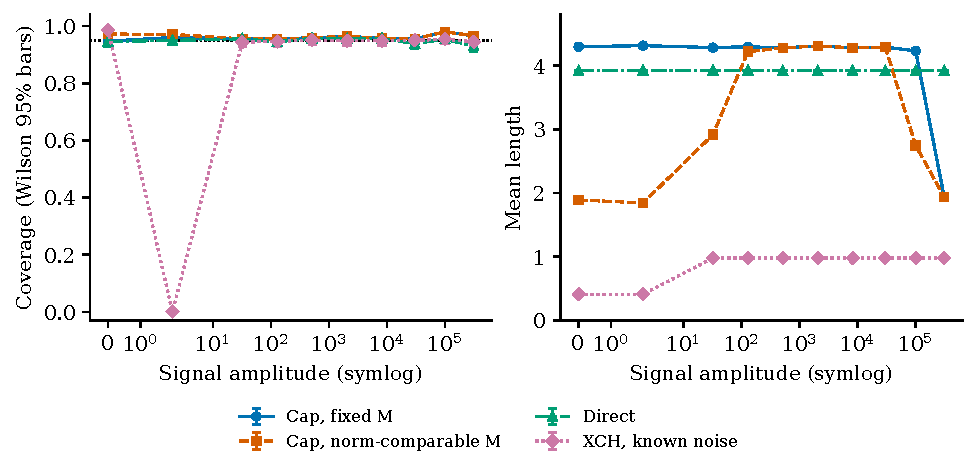
\includegraphics[width=\textwidth]{../figures/02_fixed_budget.pdf}
\caption{Paired fixed-budget and norm-comparable signal sweeps at $p=16$, cap one and $\tau=1$, with 1,000 new datasets per amplitude. The fixed budget is $342023.69$ throughout. Bars are Wilson 95\% coverage intervals or 1.96 standard errors for mean length. XCH is not guaranteed over the weak-signal cap union.}\label{fig:signal}
\end{figure}
\paragraph{Pointwise precision and scalar loss.}
In the four new $p=32,64$ cases, cap coverage ranges from 0.965 to 0.978; normalized mean lengths range from 7.20 to 8.01 times $\tau\sqrt{r/p}$. This supports the stated finite-grid behavior under deliberately strong P1 conditions, without identifying a limiting slope or optimal signal threshold. Regular XCH and the support oracle have smaller constants here.

The saved S03\_002 midpoint MSE is 12,084,661.379, with one sentinel event among 500 draws. The R1 companion on the same observations has MSE 0.148 (standard error 0.025), below its uniform theoretical bound 9.601. All sentinel observations remain in the loss calculation, and every interval endpoint is unchanged. The old midpoint is retained as a diagnostic, never relabeled as the R1 estimator.
\begin{figure}[t]\centering
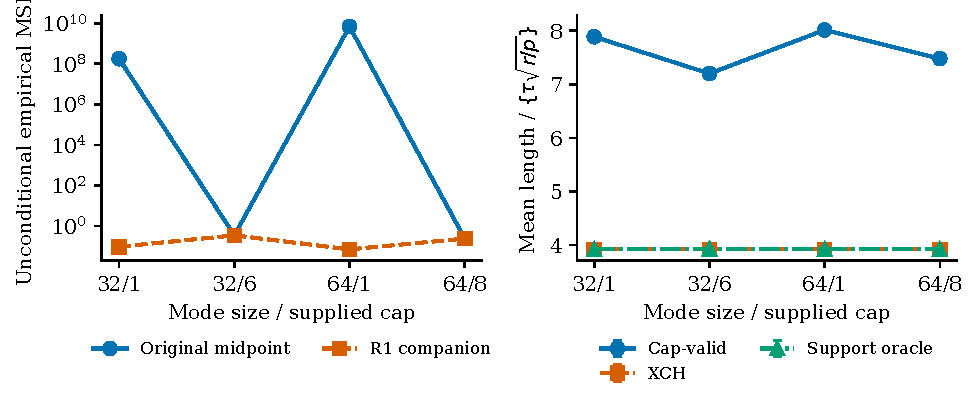
\includegraphics[width=\textwidth]{../figures/04_scalar_and_pointwise.pdf}
\caption{Strong saturated cases with 1,000 new datasets each. Left: unconditional empirical MSE including rare sentinel losses; the scalar correction leaves confidence intervals unchanged. Right: length divided by $\tau\sqrt{r/p}$, with 1.96 standard errors. The logarithmic MSE display does not assert precise estimation of rare-loss expectations; all raw losses and their uncertainty are retained.}\label{fig:pointwise}
\end{figure}
\paragraph{Calibration and assumption violations.}
All 18 within-cap whole-replicate corruption cases have median-interval coverage 1.000 in 1,000 trials each, with conservative lengths; the deliberately violated 120-row/zero-supplied-cap case has coverage 0.000. For $m=1,n=2,\sigma=1$, independent upper-scale calibration has coverage 0.995 versus 0.703 for the naive plug-in. Gaussian residual independence and the chi-square degrees of freedom are part of the experiment, not assumed for arbitrary noise. Fourth-moment-based MSE error bars are not asserted for the heavy-tail cases.

\paragraph{Optimization and input cost.}
V02 fixes the arbitrary loading, signal direction, norm budget, noise and tolerance across all budgets. Of 600 solves, 7 meet endpoint tolerance $0.05$, all at the largest budget and strongest amplitude; 593 remain unresolved. Mean gaps at 3,000 nodes range from 0.127 to 0.353. All feasible-witness gaps are finite and retained, including failures. These guarded float64 outer bounds do not implement the ideal high-dimensional minimax estimator. Fresh timings of the revised public scalar/interval interface use one thread, one warmup and ten calls per dimension; $p=64$ requires 2,097,152 input bytes and averages 0.0876 seconds per call. Traced allocations exclude the preallocated input and potentially untraced native workspace.

The XCH comparison is a local implementation of the tensor-PCA procedure in Section 4.2 of \citet{xu2025}: HOSVD initialization and two simultaneous projection updates, with known-noise and residual plug-in scales. Its regular-stratum theorem requires more than correct rank. Zero and rank-mismatched cases are explicitly outside the specified model; initialization, alignment and remainder constants are not certified for the other individual cases. No inference of finite-sample cap-uniform coverage or leading-constant dominance is made from these comparisons.
